\documentclass[slovene]{book}
\usepackage{amsmath} 
\usepackage{amssymb} 
\usepackage{makeidx} 
\usepackage{graphicx} 
\usepackage{epstopdf}
\graphicspath{{img/}}

\usepackage{url}
\usepackage{babel}
%\usepackage[T1]{fontenc}
\usepackage[cp1250]{inputenc}
\usepackage{color}
\usepackage[normalem]{ulem}
% define red
\newcommand{\red}[1]{\textcolor{red}{#1}}

%\includeonly{chaptr2} %If you just want to process chaptr2.tex

%%%
% new commands
%%%

\newcommand{\eng}[1]{(angl.~\emph{#1})}

%%%
% definicija
%%%

\newtheorem{definicija}{Definicija}

%%%
% Zgled
%%%

\newtheorem{zgled}{Zgled}

%%%
% document
%%%

\begin{document}

\author{Uredil prof. dr. Miha Mraz}
\title{Analiza zmogljivosti obla�nih in stre�ni�kih storitev}
\date{Maj 2015}
\maketitle

\frontmatter
\tableofcontents

\chapter{Predgovor}


Pri�ujo�i uvod bom napisal naknadno.


prof.dr. Miha Mraz, Ljubljana maj 2015



\mainmatter

\chapter[Zmogljivst Beowulf gru�e Raspberry Pi ra�unalnikov \\ (G. Vitek,  �. Pal�i�, M. Smerkol)]{Zmogljivst Beowulf gru�e Raspberry Pi ra�unalnikov}
\huge Gregor Vitek, �an Pal�i�, Maj Smerkol\\
\normalsize
\bigskip

\section{Uvod}

Na spletu lahko najdemo �e opravljene znane benchmarke\cite{4Benchmarks}, ki ocenjujejo dolo�ene lastnosti obla�nih sistemov (S2). Tu lahko najdemo podatke o procesni mo�i sistema, ki ga dobimo v uporabo, koli�ini pomnilnika na tak�nem sistemu in zmogljivosti opravljanja nekaterih znanih testov, kot so naprimer urejanje velike koli�ine podatkov. Te meritve, ki jih lahko preberemo med �e opravljenimi testi, pa ne ka�ejo na zmogljivost neke dolo�ene storitve, kot jo do�ivlja uporabnik, ampak samo povejo, kako zmogljiva je strojna oprema, ki jo dobimo na voljo. Kon�nega uporabnika storitve ponavadi zanima predvsem hitrost odzivanja, ki je odvisna od ve� parametrov.
Med slednje spadajo hitrost in latenca povezave od naprave uporabnika (angl. \textit{end point}) do fizi�ne lokacije obla�ne storitve ali stre�nika, velikost poslanega zahtevka, hitrost odbelave zahtevka, hitrost in latenca poslanega odgovora iz oblaka ali stre�nika proti uporabniku in drugo. Pri tem lahko lahko nekatere storitve implementiramo na tak na�in, da uporabnik verjame, da je odzivni �as veliko manj�i, kot dejansko je (naprimer shranjevanje datotek na disk v oblaku). Na kon�no uporabnikovo izku�njo hitrosti vpliva tudi zmogljivost naprave, ki predstavlja njegovo dostopno to�ko. 

Kot omenjeno zgoraj se na spletu najdejo seznami spletnih sistemov, ki jih lahko uporabniki med seboj primerjajo. Primerjajo lahko rezultate za razli�ne parametre kot so hitrost procesorja pri ra�unanju s plavajo�o vejico ali celimi �tevili, hitrost prenosa pri branju podatkov oz. pisanju na pomnilnih enotah, hitrost prenosa podatkov lokalno znotraj obla�ne storitve in drugo. Pri testiranju teh parametrov se lahko uporabi razli�na orodja kot so SPEC CPU 2006, Test Harness, TeraSort, Geekbench in �e mnogo drugih. Pri sami izbiri programov se moramo osredoto�iti tudi na bremena, ki jih lahko s posameznim programom definiramo in tako testiramo �eljene parametre. Klju�en kriterij poleg kakovosti storitev in definiranje bremen je tudi cena. Za�eljeni so prosto dostopni oz. zastonjski progami. 

Pri testiranju spletnih stre�nikov (S1) uporabnika navadno zanima �tevilo zahtev, ki jih stre�nik obdela, latenca oz. �as odziva stre�nika za novo povezavo ali zahtevek, in koli�ina prenesenih podatkov v sekundi, glede na razli�ne parametre (velikost, shranjevanje v predpomnilnik, razli�na pasovna �irina). Za izvajanje stresnih testov se na spletu nahaja veliko orodij, ki lahko pridejo v pomo� (Apachech, Apache JMeter, Curl-loader, OpenSTA). 

\subsection{Znanje}

Sistem, ki ga bomo testirali, smo izbrali na podlagi svojega znanja in zanimanja. 
�lani te skupine imamo predznanje iz arhitekture in organizacije ra�unalni�kih sistemov, kot so procesne enote, pomnilni�ka hierarhija in vhodno/izhodne naprave. Poznamo tudi paralelno programiranje na razli�nih platformah v jeziku C, kar bi nam lahko pomagalo pri optimizaciji dolo�enih storitev. Imamo predznanje iz stre�ni�kih arhitektur in osnov spletne komunikacije. Imamo tudi omejene izku�nje uporabe PaaS (angl. \textit{platform as a service}) za postavitev spletnih strani in postavitve podakovnih baz na teh stre�nikih. Nimamo pa izku�enj s testiranjem in merjenjem zmogljivosti katerega koli on na�tetih modelov.

\begin{figure}[htbf]
\centerline{\includegraphics[scale=0.5]
{4_vzorec.eps}}
\caption{Odvisnost izbire S1 in S2 glede na podane atribute.}
\label{fig:miselni}
\end{figure}

\subsection{Izbira ciljnih sistemov}

Za ciljni sistem bi lahko izbrali kak�nega od ve�jih ponudnikov obla�nih storitev kot so Google Cloud, Amazon web service, Microsoft Azure, lahko tudi kak�nega manj�ega, naprimer Rackspace. Ve�ina teh ponudnikov ima omejene zastonjska testna obdobja, med katerimi bi lahko izvedli meritve.
Ker imamo dostop do ra�unalnika Raspberry Pi \footnote{http://www.raspberrypi.org/} in predvsem zastonjskih verzij obla�nih storitev, nas zanima primerjava med temi platformami. Raspberry Pi je ra�unalnik, ki stane okrog 30 evrov in ne porabi prakti�no ni� elektrike, v zameno pa ponuja primerno majhno zmogljivost. Ne pla�ljive obla�ne storitve so mo�no �asovno omejene ali pa ponujajo prav tako zelo majhne zmogljivosti.
Zaradi na�ih predznanj lahko storitev za stre�nik (glej sliko \ref{fig:miselni}), katerega ustroj in delovanje poznamo, bolje optimiziramo, kot obla�no storitev, kar je prav tako vredno preveriti.

Ker pa je implementacija optimizirane storitve in postavitev lastne gru�e relativno zahtevno opravilo, mi pa imamo na voljo omejen �as, smo se odlo�ili za testiranje zmogljivosti gru�e ra�unalnikov Raspberry Pi. Le ti so se v zadnjem �asu zaradi nizke cene na mnogih podro�jih ra�unalni�tva za�eli uporabljati. Nas zanima, ali so ra�unalniki tak�nega tipa primerni tudi za uporabo na podro�jih, ki zahtevajo ra�unsko mo�. Na podlagi izmerjenih rezultatov lahko primerjamo zmogljivost z druga�nimi sistemi, na katerih so meritve �e opravljene. Prav tako lahko nadaljujemo raziskovanje na tem podro�ju z poskusom optimizacije enake storitve na druga�nem sistemu v prihodnosti.

\subsection{Breme in cilj primerjave}

Za storitev, ki jo bo na�a gru�a ponujala, smo izbrali manipulacijo nad frekven�nim spektrom avdio datotek. To pomeni, da smo implementirali porazdeljen algoritem FFT, ki pretvori datoteko iz vzor�nega prostora v frekve�ni spekter, nato nad tem opravimo preprosto operacijo, na primer zamik v vi�je frekvence, nato pa z inverznim FFT spet naredimo datoteko v vzor�nem prostoru.

Bremena so tako razli�no velike zvo�ne datoteke. Ker na� spletni stre�nik, ki to storitev ponuja, sprejme eno ali ve� datotek, testiramo tudi izvajanje ve�ih instanc algoritma hkrati.

Cilj primerjave je ugotoviti, ali je ra�unalnik Raspberry Pi primeren za postavitev gru�e, ki bo izvajala ra�unsko zahtevne storitve. Da bi to ugotovili, moramo primerjati �as izvajanja na procesorju, �as latence oddaljenega sistema prek medmre�ja in �as po�iljanja podatkov po gru�i.

\section{Sistem}

%%%%%%%%%%%%%%%%%%% FOTOGRAFIJA %%%%%%%%%%%%%%%%%%%%%%%%
\begin{figure}[H]
\centerline{\includegraphics[scale=0.1]
{4_foto.eps}}
\caption{Fotografija gru�e. Na levi je 100 megabitno stikalo, na desni pa ra�unalniki Raspberry Pi na pladnju.}
\label{fig:foto}
\end{figure}

Na� sistem je gru�a ra�unalnikov, narejena po vzoru Beowulf gru� (glej sliko \ref{fig:foto}). Namenjena je zaganjanju porazdeljenih programov. V mre�o smo povezali �tiri ra�unalnike Raspberry Pi, model 1B, tri modele 1B+. Povezani so v gru�o s pomo�jo knji�njice MPI\footnote{Message Passing Interface, knji�njica za medprocesno komunikacijo prek omre�ja ali na lokalnem ra�unalnikom}. Do njega imamo SSH dostop tudi z zunanjega omre�ja. Storitev je dostopna prek stre�nika, ki smo ga implementirali sami. Programska koda stre�nika in implementacije algoritma FFT je v prilogi.

\begin{figure}[H]
\centerline{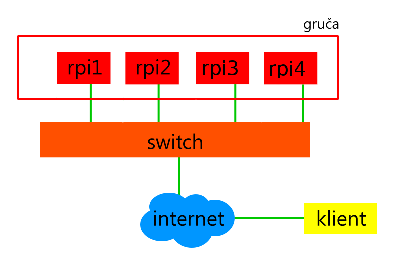
\includegraphics[scale=1.5]
{4_shemaSistema.eps}}
\caption{Shema sistema. Rde�i kvadrati so ra�unalniki Raspberry Pi.}
\label{fig:gruca}
\end{figure}

Do tega sistema dostopamo s klienti, ki so izven lokalnega omre�ja (glej sliko \ref{fig:gruca}). Gru�o uporabljamo kot ra�unski stre�nik, ki po zahtevi klienta izvaja porazdeljeno hitro Fourierjevo transformacijo. Klient prek omre�ja po�lje podatke v obliki glasbene datoteke, gru�a pa podatke sprejme (to stori stre�nik, ki te�e na master ra�unalniku gru�e) in izvajanje algoritma porazdeli prek vseh ra�unalnikov v gru�i, vklju�no s sabo.

Gru�a se nahaja na Velikem Lo�niku, na omre�ju Telekoma. Dostopna je prek �irokopasovne povezave po opti�nem kablu (angl. \textit{FTTH - fiber to the home}) s hitrostjo 20Mb/s v obe smeri. Vse povezave po hi�i so po bakreni parici kategorije 6, omre�na oprema pa je prepustna najmanj 100Mb/s.

V za�etku smo testirali dostop do gru�e od zunaj in delovanje sistema MPI na ra�unalniku rpi1. To smo storili tako, da smo na njem poganjali z MPI implementiran algoritem porazdeljeni Quicksort (porazdeljeno hitro urejanje\footnote{http://en.wikipedia.org/wiki/Quicksort\#Parallelization}).

Pri povezovanju Raspberry Pi-jev v gru�o smo uporabili Message Passing Interface(MPI), ki je standard za izmenjevanje sporo�il med ra�unalniki oz. procesih v ve�-ra�unalni�kih sistemih, gru�ah in delovnih postajah. Omogo�a komunikacijo to�ka-to�ka, skupinske komunikacije, spremljanje delovanja in tudi spreminjanje topologije za posamezen program. MPI je standard, ki omogo�a velik nabor funkcij, vendar za uporabo standarda ni potrebno poznati vseh. Pri sami komunikaciji ra�unalniki med seboj uporabljajo implementacijo MPICH2 \cite{4Mpich},
ki je zelo raz�irjena programska knji�nica, ki je enostavna za vzpostavitev in uporabo. Na vsakem ra�unalniku je implementacija 
MPICH2 in datoteka (machinefile)\cite{4Gruca}, v kateri so zapisani IP naslovi sodelojo�ih (sosednjih) lokalnih ra�unalnikov, na katere se delo porazdeli.

Implementirali smo porazdeljeni algoritem FFT, ki se izvaja na gru�i. 

\subsection{Implementacija storitve}

V gru�o smo dodali ve� ra�unalnikov, da je prava gru�a, ne le en ra�unalnik, na katerem te�e MPI. Raspberry Pi smo pripravili na delovanje v gru�i tako, da smo klonirali sliko datote�nega sistema. Potrebni so bili popravki v konfiguraciji omre�ja in sprememba hostname-a vsakega ra�unalnika. Po tem je gru�a delovala brez te�av.

Implementirali smo storitev, ki zvo�no datoteko pretvori v binarno s pomo�jo knji�njice \texttt{libsndfile}\cite{4Audio}. Testiranje smo izvedli z zvo�no datoteko, veliko pribli�no 8 miljonov vzorcev (okrog 3 minute zvoka, nekompresirana velikost je okrog 15MB). Program na enem jedru te�e zelo po�asi. Ni se izpolnil strah, da bi algoritem tekel prehitro, da bi se ga izpla�alo poganjati na gru�i. Imeli smo nekaj te�av s kodiranjem datoteke nazaj v zvo�no datoteko.

Pretvorbo izvajamo z rekurzivnim algoritmom FFT. Implementacija je zaradi uporabe razreda ValArray iz knji�njice STL po�asna, �e je prevanjanje izvedeno z Microsoft Visual Studio prevajalnikom. Program, ki se izvaja na gru�i, na kateri te�e Linux (distribucija Arch Linux), je preveden s prevajalnikov gcc, ki se v tem primeru obna�a veliko bolje - koda se izvaja hitreje.

\vspace{10pt}

Implementirali smo stre�nik, ki sprejema zahtevke z eno ali ve� datotekami in nato odgovori. Implementirali smo tudi klienta, ki po�ilja zahtevek z eno ali ve� datotekami in sprejme odgovor stre�nika.

Program, ki izvaja manipulacije frekven�nega spektra, upo�teva lastnosti hitre Fourierjeve transformacije in pravilno obdeluje zvok. Zavr�emo del frekven�nega spektra, ki je zrcalna slika relevantnega dela. Transformacije, ki jih izvajamo na preostanku, so zato smiselne in se obna�ajo kot pri�akovano.

\vspace{10pt}

% povezovanje v enoten sistem

\section{Meritve}

Na� problem predstavlja veliko ra�unsko breme gru�i ampak relativno majhno breme za prenos podatkov prek omre�ja. Na enem vozli��u traja obdelovanje 5 sekund zvoka okrog 40 sekund. Algoritem je hitrostnega razreda $O(n * log(n))$.

Zaradi tipa problema in bremena nas zanimajo �asi ra�unanja (procesiranja na gru�i, wall-clock time, v odvisnosti od �tevila uporabljenih vozli�� in velikosti bremena), prenosa podatkov na in iz gru�e (latenca omre�ja - �as prenosa je najbr� zanemarljiv, saj so datoteke velike med 1MB in 15MB), latence prenosa podatkov med vozli��i v gru�i (da vidimo, ali je paralelizacija na gru�i primerna ali bi bilo bolje uporabljati paralelizacijo na ve� jedrih ali podobni arhitekturi) in najve�je �tevilo datotek, ki jih lahko obdeluje hkrati, preden se gru�a ali deli nje sesujejo.

Izvajamo ve� meritev:
\begin{itemize}
\item celoten �as izvajanja storitve od trenutka, ko klient za�ne po�iljati podatke, do trenutka, ko se do konca prenese odgovor stre�nika.
\item �as izvajanja ra�unskega dela storitve od klica programa FFT do konca njegovega izvajanja.
\item �as prejemanja in po�iljanja podatkov prek omre�ja.
\item �as po�iljanja podatkov med ra�unalniki v gru�i po lokalnem omre�ju (klici funkcij MPI scatter in MPI gather.
\item skupna hitrost obdelava podatkov v bajtih na sekundo.
\end{itemize}

Meritev �asa izvajanja ra�unanja in meritev �asa prenosa podatkov med procesi smo ponovili tudi na ra�unalniku s procesorjem Intel i5-3317U, s frekvenco ure 1,7GHz in 4GB DDR3 delovnega spomina in 3MB L3 cache-a. Pri tem smo program izvajali lokalno, brez stre�nika. Rezultati nam dajo primerjavo med ve�jedrnim procesorjem s hyperthreadingom in gru�o enojedrnih. Bralec lahko primerja tudi zmogljivost glede na ceno, pri �imer mora vedeti, da ra�unalnik Raspberry Pi stane okrog 30 evrov, stikalo, ki smo ga uporabili, stane 40 evrov do 100 evrov, ra�unalnik z Intelovim procesorjem, ki smo ga uporabili, pa okrog 800 evrov.

%%% TODO ker swittch mamo

Mertive smo izvedli na 1, 2 in 4 ra�unalnikih v gru�i. Izvedli smo teste z enim 1, 5, 20, 60 in 180 sekund dolgo vhodno zvo�no datoteko in z 1, 5 in 10 vhodnimi datotekami velikosti 5 sekund. Posebej smo testirali �e ve� datotek po 180 sekund, s �imer smo uspeli sesuti gru�o.

Zaradi zelo dolgega �asa izvajanja storitve za datoteke, dolge 180s, smo to meritev izvajali le na vseh 4 ra�unalnikih v gru�i in na procesorju Intel i5.

Vse teste smo ponovili trikrat.  

%%======================== konst num = 1, var size =======================
%%============================= �as zahtevka =============================

\subsection{Izmerjeni �asi: 1 datoteka, razli�ne velikosti datoteke}
Meritev celotnega �asa izvajanja storitve od trenutka, ko klient za�ne po�iljati podatke, do trenutka, ko se do konca prenese odgovor stre�nika. 
\begin{table}[h]
\begin{tabular}{l|ccccc}
RPIs & n[s] = 1  & n[s] = 5  & n[s] = 20  & n[s] = 60  & n[s] = 180 \\ \cline{1-6}
1    & 6,36      &    21,85  &    86,11   &   359,54   & -          \\
     & 6,23      &    20,70  &    85,98   &   361,90   & -          \\
     & 6,48      &    21,73  &    84,97   &   363,97   & -          \\ \cline{1-6}

2    & 5,27      &    14,50  &    44,69   &   179,31   &  -         \\
     & 5,23      &    14,08  &    48,99   &   179,84   &  -         \\
     & 5,20      &    13,08  &    48,35   &   178,99   &  -         \\ \cline{1-6}

4    & 8,26      &    10,67  &    27,85   &    94,49   &    193,99  \\
     & 9,31      &    10,66  &    28,50   &    93,18   &    203,01  \\
     & 9,34      &    11,06  &    27,15   &    97,29   &    201,75  \\
\end{tabular}
\caption{Tabela izmerjenih vrednosti �asa izvajanja celotnega zahtevka.}
\end{table}

\begin{figure}[H]
\centerline{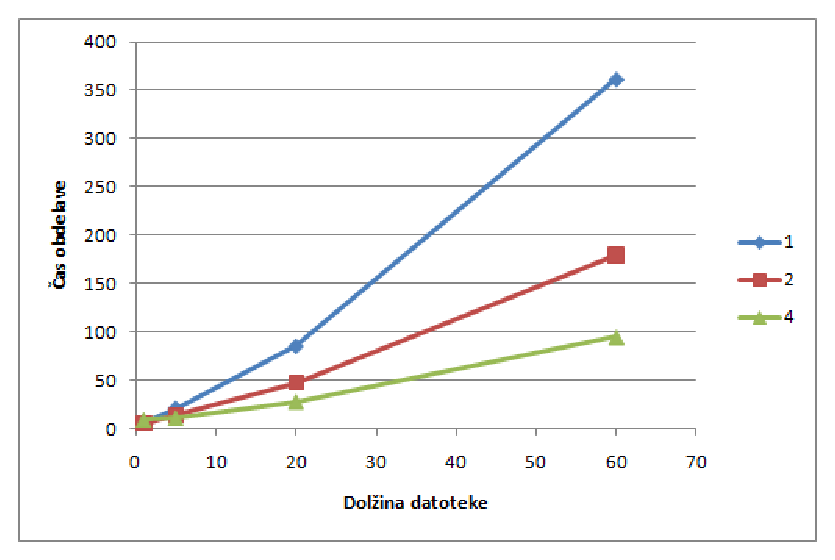
\includegraphics[scale=1]
{4_dolzinaDatotek.eps}}
\caption{Graf �asa celotnega izvajanja zahtevka.}
\label{fig:zahtevek1}
\end{figure}

Na grafu \ref{zahtevek1} vidimo, da se, ko podvojimo �tevilo vozli�� v gru�i, �as izvajanja v skoraj razpolovi. Iz grafa \ref{casfft1} lahko vidimo, da je razlika med linearno pohitritvijo in dose�eno pohitritvijo predvsem posledica dalj�ega prenosa podatkov prek omre�ja, ki seveda ni odvisen od velikosti gru�e.

%%%%%%%%%%%%%%%%%%%%%%%%%%%%%%%%% �AS OMRE�JA V SEKUNDAH ZA 1 FAJL

\subsection{Izmerjeni �asi prenosa podatkov in re�ije (angl. \textit{overhead}) v sekundah: 1 datoteka, razli�ne velikosti datoteke}

\begin{table}[h]
\begin{tabular}{l|ccccc}
RPIs & n[s] = 1  & n[s] = 5  & n[s] = 20  & n[s] = 60  & n[s] = 180 \\ \cline{1-6}
1    & 0,17      & 0,29      & 1,57       & 4,40       &  -         \\
     & 0,12      & 0,36      & 1,24       & 3,83       &  -         \\
     & 0,12      & 0,35      & 1,09       & 3,82       &  -         \\ \cline{1-6}

2    & 0,13      & 0,34      & 1,28       & 3,79       &  -         \\
     & 0,12      & 0,34      & 1,47       & 4,16       &  -         \\
     & 0,15      &  0,68     & 1,12       & 3,79       &  -         \\ \cline{1-6}

4    &  0,66     &  1,59     &  5,25      &  4,35      &  17,96     \\
     &  0,46     &  4,65     &  7,90      &  8,32      &  20,09     \\
     &  0,78     &  2,06     &  8,32      &  7,39      &  19,61     \\ %% idelno ponoviti tretjo meritev za 180 - net zajbava
\end{tabular}
\caption{Tabela izmerjenih vrednosti �asa prenosa podatkov na prek omre�ja na gru�o.}
\end{table}



%%================================ hitrost ra�unanja ============================= bajti na service

\subsection{Izmerjena hitrost obdelave podatkov v kB/s: 1 datoteka, razli�ne velikosti datoteke}

\begin{table}[h]
\begin{tabular}{l|cccc}
RPIs & n[s] = 1  & n[s] = 5  & n[s] = 20  & n[s] = 60  \\ \cline{1-6}
1    & 9636      & 19781     & 20137      & 14434      \\
     & 10871     & 18099     & 20684      & 14948      \\
     & 10872     & 18872     & 20245      & 14863      \\ \cline{1-6}
                                                       
2    & 14429     & 33045     & 38939      & 30263      \\
     & 12404     & 30738     & 37932      & 29522      \\
     & 14356     & 32215     & 39086      & 29255      \\ \cline{1-6}
                                                       
4    &  17298    &  47105    &  70233     & 57326      \\
     &  17392    &  45511    &  70452     & 56347      \\
     &  17230    &  47181    &  70283     & 58203      \\
\end{tabular}
\caption{Tabela izmerjenih vrednosti hitrosti obdelave podatkov. n[s] je dol�ina zvo�ne datoteke v sekundah, RPIs pomeni �tevilo vozli�� v gru�i.}
\end{table}

\begin{figure}[H]
\centerline{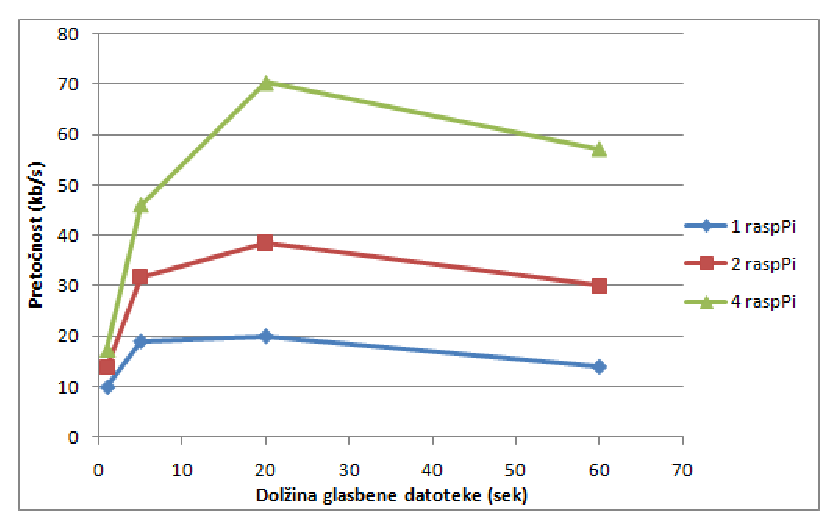
\includegraphics[scale=1]
{4_pretocnost.eps}}
\caption{Graf hitrosti obdelave podatkov.}
\label{fig:pretocnost}
\end{figure}

Na grafu \ref{fig:pretocnost} vidimo primerjave hitrosti obdelave podatkov za celotno storitev (velikost datoteke v kilobajtih deljena s �asom, kot ga vidi klient). Zanimivo je, da je o�itno okrog datotek velikosti 20 sekund optimalna to�ka, pri kateri se �asi obdelave podatkov, prenosa podatkov in latenca omre�ja pridejo v za uporabnika najbolj�e razmerje. Lahko razberemo tudi, da je hitrost obdelave odvisno skoraj linearno od �tevila ra�unalnikov v sistemu. To pomeni, da �e nismo dosegli maksimalne pohitritve po Amdahlovem zakonu in bi s podvojitvijo �tevila ra�unalnikov lahko �e vsaj enkrat podvojili zmogljivost gru�e.


%%%%%%%%%%%%%%%%%%%%%% FFT �AS NA GRU�I
\subsection{Izmerjen �as ra�unananja FFT v sekundah: 1 datoteka, razli�ne velikosti datoteke}

\begin{table}[h]
\begin{tabular}{l|ccccc}
RPIs & n[s] = 1  & n[s] = 5  & n[s] = 20  & n[s] = 60      \\ \cline{1-6}
1    & 4,71      & 18,16     & 82,15      & 357,95         \\
     & 5,15      & 18,70     & 79,56      & 345,43         \\
     & 4,26      & 19,90     & 82,18      & 348,29         \\ \cline{1-6}

2    & 2,16      & 9,23      & 39,93      & 166,33         \\
     & 2,15      & 9,64      & 41,16      & 171,19         \\
     & 2,12      & 9,24      & 39,71      & 173,15         \\ \cline{1-6}

4    &   1,13    &  4,65    &  19,45      & 84,26          \\
     &   1,11    &  4,54    &  19,98      & 85,31          \\
     &   1,07    &  4,67    &  19,47      & 82,40          \\
\end{tabular}
\caption{Tabela izmerjenih vrednosti �asa izvajanja algoritma FFT. n[s] pomeni dol�ina zvo�ne datoteke v sekundah, RPIs pa �tevilo vozli�� v gru�i.}
\end{table}

V tabeli lahko vidimo, da je pohitritev pri dodajanju vozli�� v gru�o superlinearna. To se pri porazdeljevanju programa skoraj nikoli ne zgodi. V na�em primeru je do tega pri�lo, ker nalogo nazdelimo na manj�e podprobleme na druga�en na�in, kot je to standardno pri FFT. Ponavadi se pri FFT zvo�no datoteko razdeli na lihe in sode vzorce, mi pa smo celotno datoteko razdelili na ve� manj�ih. Ob tem sicer izgubimo na kvaliteti zvoka, vendar to zaradi velikosti datotek ni problemati�no, saj se v praksi ponavadi stori isto, vendar na �e mnogo ve� mnogo manj�ih kosov, kot smo to storili mi. Razlika v kvaliteti zvoka ni opazna za �loveka. Rezlutat tega je, da zahtevnost algoritma pade in pride do rahlo superliearne pohitritve. Glej poglavje zaklju�ek \ref{sec:zakljucek}. 

%%%%%%%%%%%%%%%%%%% FFT �AS NA INTELU
\subsection{�as izvajanja algoritma FFT na ra�unalniku s procesorjem i5, za primerjavo ra�unske zmogljivosti}

\begin{table}[h]
\begin{tabular}{l|ccccc}
�t. jeder & n[s] = 1  & n[s] = 5  & n[s] = 20  & n[s] = 60  & n[s] = 180 \\ \cline{1-6}
1    & 1,15      & 4,84      & 21,56      & 86,54      & 133,01     \\
     & 1,07      & 4,76      & 19,74      & 86,91      & 187,35     \\
     & 1,07      & 4,57      & 17,65      & 86,50      & 179,31     \\ \cline{1-6}

2    & 0,79      & 3,33      & 12,89      & 50,69      & 112,80     \\
     & 0,63      & 2,63      & 11,51      & 49,31      & 73,87      \\
     & 0,66      & 2,74      & 11,26      & 48,28      & 107,95     \\ \cline{1-6}
 
4    & 0,50      & 1,87      & 7,85       & 33,92      & 71,17      \\
     & 0,41      & 1,76      & 7,38       & 31,56      & 68,11      \\
     & 0,46      & 1,84      & 7,43       & 31,46      & 66,88      \\
\end{tabular}
\end{table}

\begin{figure}[H]
\centerline{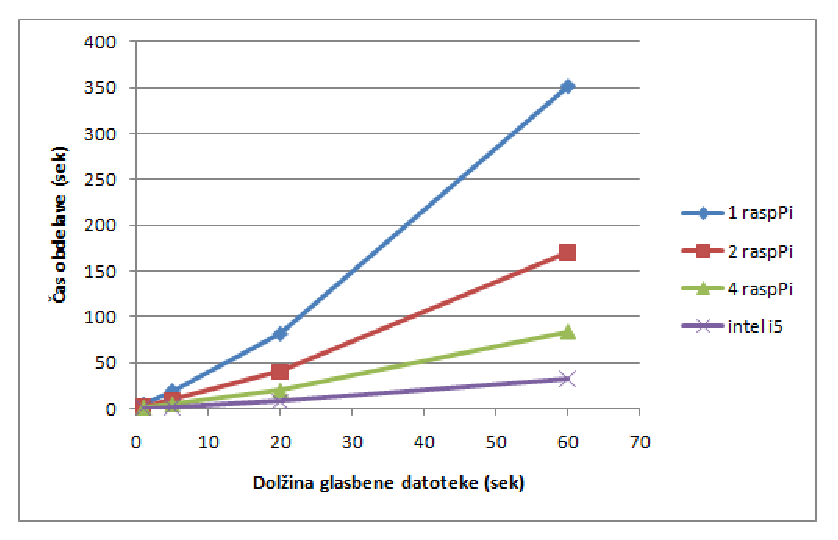
\includegraphics[scale=1]
{4_obdelava.eps}}
\caption{Graf �asov izvajanja obdelave podatkov.}
\label{fig:obdelava}
\end{figure}

Na grafu \ref{fig:obdelava} vidimo primerjavo �asov izvajanja algoritma FFT. Na abscisni osi so razli�ne dol�ine datotek, na ordinatni pa �as izvajanja. Skala je povsod linearna. Razli�ni grafi predstavljajo meritve razli�nih konfiguracij sistema. Najhitrej�i, ozna�en kot Intel i5, je en dvojedrni procesor s hyperthreadingom. Glede na celotno ceno sistema se gru�a izka�e za bolj�o re�itev.
Zanimiva je tudi primerjava med gru�o z razli�nim �tevilom vozli��, saj je pohitritev prakti�no linearno odvisna od �tevila vozli�� v gru�i.





















































%%%====================== konst size = 5s, var num =======================
%%============================= �as zahtevka =============================
%\iffalse

\subsection{Izmerjeni �asi izvajanja celotnega zahtevka: datoteka dolga 5s, razli�no �tevilo datotek v zahtevku}

\begin{table}[h]
\begin{tabular}{l|ccc }
RPIs & N[f] = 1 & N[f] = 5 & N[f] = 10 \\ \cline{1-4}
1    & 21,85 & 102,38 & 208,68 \\
     & 20,70 & 104,35 & 203,89 \\
     & 21,73 & 103,75 & 218,35 \\ \cline{1-4}

2    & 14,50 &  70,95 & 126,58 \\
     & 14,08 &  70,32 & 150,61 \\
     & 13,08 &  71,55 & 129,25 \\ \cline{1-4}

4    & 10,67 &  55,44 &  98,99 \\
     & 10,66 &  55,93 &  95,94 \\
     & 11,06 &  55,80 &  95,94 \\
\end{tabular}
\caption{Tabela izmerjenih vrednosti celotnega izvajanja zahtevka. N[f] pomeni �tevilo zvo�nih datoteke dol�ine 5 sekund, RPIs pa �tevilo vozli�� v gru�i.}
\end{table}

\begin{figure}[H]
\centerline{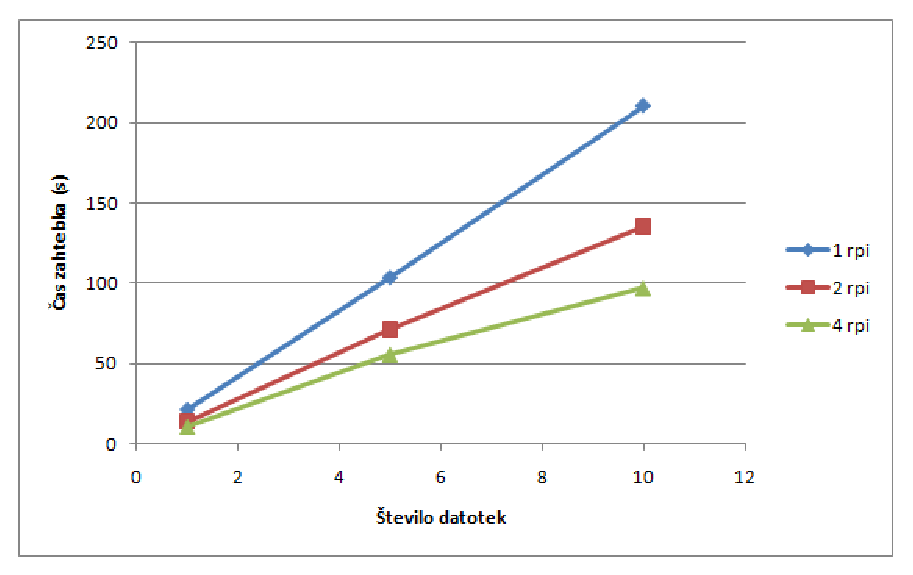
\includegraphics[scale=1]
{4_razlicnoSteviloDatotek.eps}}
\caption{Graf �asov izvajanja celotnega zahtevka za ve� datotek.}
\label{fig:obdelava}
\end{figure}

Iz grafa \ref{fig:obdelava} vidimo, da je �as izvajanja pribli�no linearno odvisen od �tevila datotek. To je razumljivo, saj gre za ve� ponovitev enakega zahtevka. �e bi �tevilo datotek zelo pove�ali, bi najbr� pri�lo do velike upo�asnitve, ko bi za�elo zmanjkovati spomina na gru�i, vendar se ob tem skoraj isto�asno tudi gru�a sesuje, ker je zaradi majhnega zunanjega pomnilnika (SSD kartica) zelo malo swap prostora, kar pomeni, da zmanjka celotnega pomnilnika skoraj isto�asno kot delovnega pomnilnika. Glej poglavje \ref{sec:zakljucek}.

%%============================= overheadm MPI graf ho�m =============================

\subsection{Izmerjeni �asi po�iljanja podatkov po gru�i: datoteka dolga 5s, razli�no �tevilo datotek v zahtevku}

\begin{table}[h]
\begin{tabular}{l|cccc}
RPIs & N[f] = 5 & N[f] = 10 \\ \cline{1-3}
1    & 0,024 & 0,047 \\
     & 0,024 & 0,048 \\
     & 0,025 & 0,048 \\ \cline{1-3}

2    & 0,542 & 1,10 \\
     & 0,548 & 1,15 \\
     & 0,549 & 1,09 \\ \cline{1-3}

4    & 0,841 & 1,64 \\
     & 0,816 & 1,63 \\
     & 0,810 & 1,69 \\
\end{tabular}
\label{mpiovermany}
\end{table}

Iz tabele \ref{mpiovermany} vidimo, da so �asi porazdelitve podatkov po gru�i (MPI scatter in gather funkciji) zelo manjhni in predstavljajo reda 1% celotnega �asa izvajanja.

%%================================ hitrost ra�unanja ============================= FFT

\subsection{Izmerjena hitrost obdelave podatkov v kB/s: datoteka dolga 5s, razli�no �tevilo datotek v zahtevku}

\begin{table}[h]
\begin{tabular}{l|cccc}
RPIs & N[f] = 5 & N[f] = 10 \\ \cline{1-3}
1    & 93,73 & 192,83 \\
     & 93,73 & 186,84 \\
     & 92,90 & 186,84 \\ \cline{1-3}

2    & 45,90 & 91,97 \\
     & 46,30 & 96,69 \\
     & 47,64 & 92,45 \\ \cline{1-3}

4    & 23,47 & 47,19 \\
     & 23,23 & 46,48 \\
     & 23,42 & 48,38 \\
\end{tabular}
\end{table}

%%================================ hitrost ra�unanja ============================= seervice

\subsection{Izmerjena hitrost obdelave podatkov v kB/s: datoteka dolga 5s, razli�no �tevilo datotek v zahtevku}

\begin{table}[h]
\begin{tabular}{l|cccc}
RPIs & N[f] = 5   & N[f] = 10  \\ \cline{1-3}
1    & 18861 & 18443 \\
     & 18789 & 18996 \\
     & 19118 & 18133 \\ \cline{1-3}

2    & 32230 & 31850 \\
     & 31792 & 30810 \\
     & 31148 & 31847 \\ \cline{1-3}

4    & 47518 & 47360 \\
     & 47514 & 47364 \\
     & 47544 & 43176 \\
\end{tabular}
\end{table}


























%\fi

\section{Zaklju�ek} \label{sec:zakljucek}

Zaradi tipa algoritma (FFT se rekurzivno deli vedno na dva dela, zato deluje dobro le, �e uporabljamo $2^n$ paralelnih niti, kar je tudi razlog, da po za�etnem poskusu nismo opravljali testov na gru�i velikosti 3.

Ker za dovolj velik $n$ velja $n*log(n) > n*log(n/m)*m$, je hitrost re�evanja problem ve�ja, �e re�ujemo ve� manj�ih problem, kot enega velikega. To je razlog, da ne porazdeljujemo po gru�i po drevesu razcepa podatkov, ki ga izvaja FFT, ampak razdelimo vse podatke na $m$ delov in nato odbelujemo vsakega posebej, pri �emer je $m$ �tevilo ra�unalnikov v gru�i. To je slaba re�itev za zelo velik $m$ ali zelo majhne zahtevke, saj bi se lahko poznala izguba kvalitete zvoka, ki jo to prinese. Razlika se na normalnih zahtevkih in na�em $m$ sicer ne pozna. Tak�en pristop se uporablja tudi v praksi, predvsem kadar se izvaja transformacije v realnem �asu (sproti).

 % 1.Poglavje

\backmatter
%\include{glossary}
%\include{notat}
\bibliographystyle{ieeetr} %The style you want to use for references.
\bibliography{mro} %The files containing all the articles and books you ever referenced.
\printindex %Make an index AUTOMATICALLY

\end{document} 
